\documentclass[10pt, aspectratio=169]{beamer}

% handout
% \documentclass[handout, 10pt]{beamer}

\usepackage{clases}

\title{Investigación Operativa}
\subtitle{Árboles}
\date{}
\author{Facundo Gutiérrez - Nazareno Faillace Mullen}
\institute{Departamento de Matemática - FCEN - UBA}
% \titlegraphic{\hfill\includegraphics[height=1.5cm]{logo.pdf}}

\newcommand \anchoPagina{1.0} % El proyector no anda bien, hay que ajustar el ancho
\begin{document}

\maketitle

\begin{frame}{Repaso de definiciones}
	\begin{minipage}{\anchoPagina \textwidth}
	
		\begin{itemize}
			\item Llamamos \textit{\'arbol} a un grafo conexo y ac\'iclico.
			\item Llamamos \textit{bosque} a un grafo ac\'iclico (unión disjunta de árboles).
			\item Llamamos \textit{hoja} a un v\'ertice de grado 1.
			
		\end{itemize}
	
	
	\begin{center}
		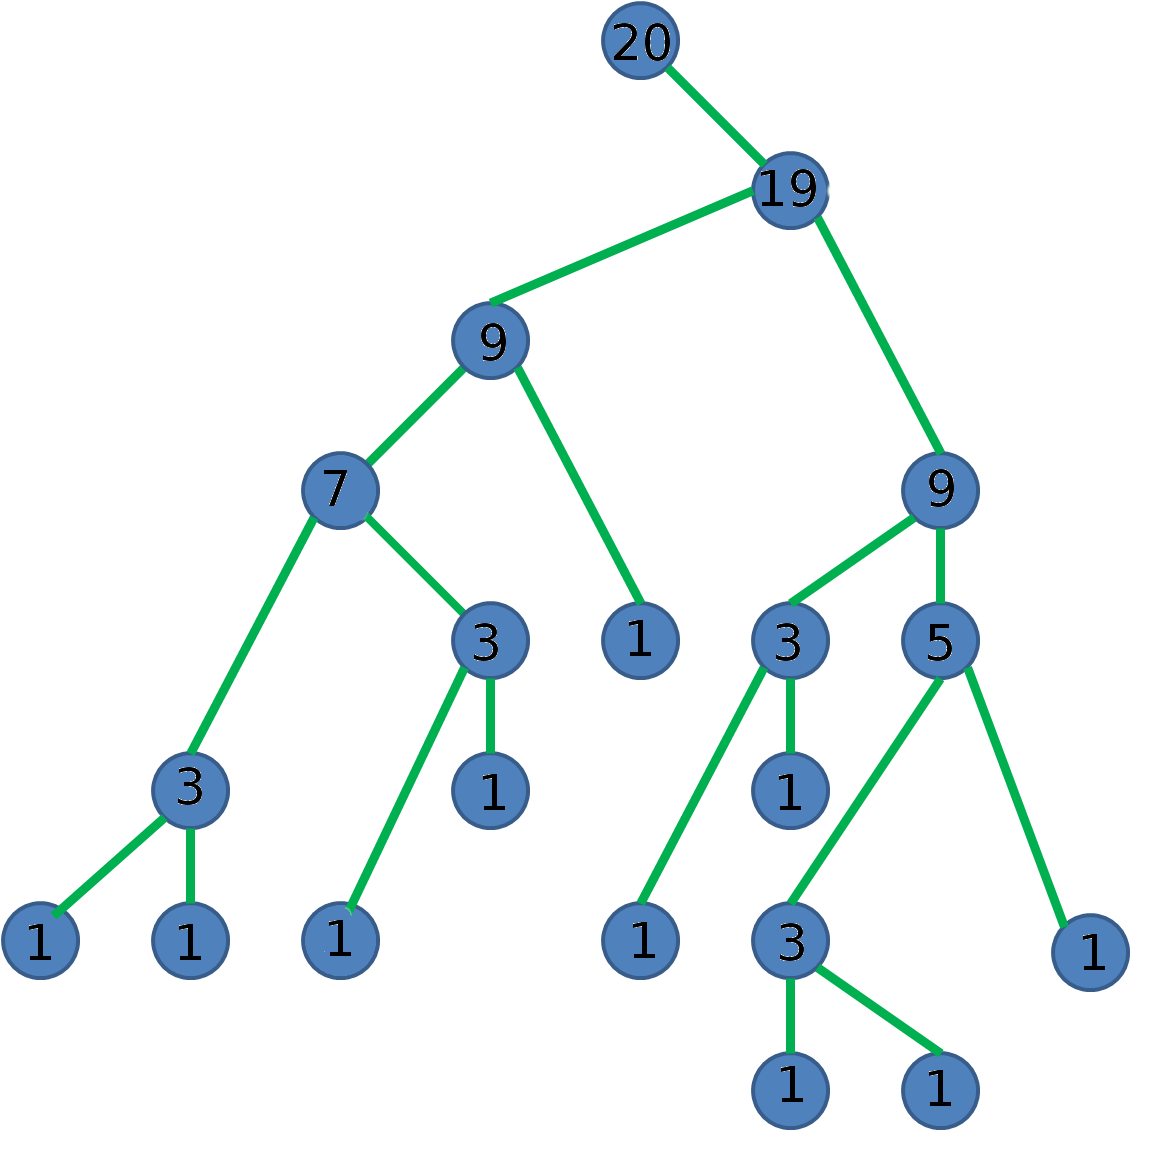
\includegraphics[scale = 0.25]{imagenes/tree.png}
	\end{center}
	\end{minipage}
\end{frame}

\begin{frame}{Ejercicio 1}
	\begin{minipage}{\anchoPagina \textwidth}
		\textbf{Proposici\'on}: Si todo v\'ertice de un grafo $\mathcal{G}$ tiene grado al menos 2, entonces $\mathcal{G}$ tiene un ciclo.	
	
		\pause
		
		\textbf{Demostraci\'on}: Supongamos que $\mathcal{G}$ no tiene ciclos. Consideremos $P$ alg\'un camino simple maximal. Sea $v$ alg\'un extremo de $P$. Como $d(v) \geq 2 \dots$ 
		
		\begin{center}
			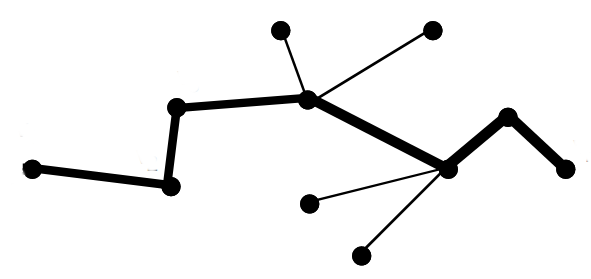
\includegraphics[scale = 0.3]{imagenes/maximal-path.png}
		\end{center} 
		\pause
		$\dots$ existe un vecino de $v$ distinto de su vecino inmediato en $P$. Llam\'emosle $w$. Si $w \in P$, entonces $\mathcal{G}$ tendr\'ia un ciclo. Si $w \notin P$, entonces podemos extender a $P$, contradiciendo su condici\'on de maximal. Concluimos que $\mathcal{G}$ necesariamente tiene un ciclo.    
			
	\end{minipage}
	
\end{frame}

\begin{frame}{Ejercicio 2}
	\begin{minipage}{\anchoPagina \textwidth}
		\textbf{Proposici\'on}: La cantidad de hojas de un \'arbol es mayor o igual al grado m\'aximo.	
		
		\pause
		
		\textbf{Demostraci\'on}: Sea $v$ un nodo de grado m\'aximo. De cada arista incidente en $v$ consideremos un camino maximal con extremo en $v$. Todos estos caminos son disjuntos (exceptuando el extremo $v$), ¿por qu\'e? \pause Porque si no fueran disjuntos, cerrar\'ian un ciclo.
		
		Razonando an\'alogamente al ejercicio anterior, podemos ver que cada extremo de estos caminos debe ser una hoja, de donde concluimos el resultado del enunciado.     
		
	\end{minipage}
	
\end{frame}



\begin{frame}{Caracterizaci\'on de un \'arbol}
	\begin{minipage}{\anchoPagina \textwidth}
	
		Son equivalentes:
		\begin{itemize}
			\item $\mathcal{G}$ es un \'arbol (conexo y ac\'iclico)
			\item Dados dos v\'ertices en $\mathcal{G}$ existe un \'unico camino que los une.
			\item $\mathcal{G} = (\mathbb{V},\mathbb{E})$ es conexo y $|\mathbb{E}| = |\mathbb{V}| - 1$
			\item $\mathcal{G} = (\mathbb{V},\mathbb{E})$ es ac\'iclico y $|\mathbb{E}| = |\mathbb{V}| - 1$
		\end{itemize}
		\pause
		¿Cu\'antas aristas tiene como m\'inimo un grafo con $c$ componentes conexas?
		\pause $|\mathbb{V}| - c$
	\end{minipage} 
\end{frame}

\begin{frame}{Ejercicio 3}
	\begin{minipage}{\anchoPagina \textwidth}
	    \small
		Un hidrocarburo saturado es una mol\'ecula $C_pH_q$ en la cual cada \'atomo de carbono tiene 4 enlaces y cada \'atomo de hidr\'ogeno tiene exactamente un enlace. Ninguna sucesi\'on de enlaces forma un ciclo.
			
		Mostrar que para todo $p \in \mathbb{Z}_{> 0}$ la \'unica forma de que un hidrocarburo saturado $C_pH_q$ exista es si $q = 2p+2$.
		\begin{center}
			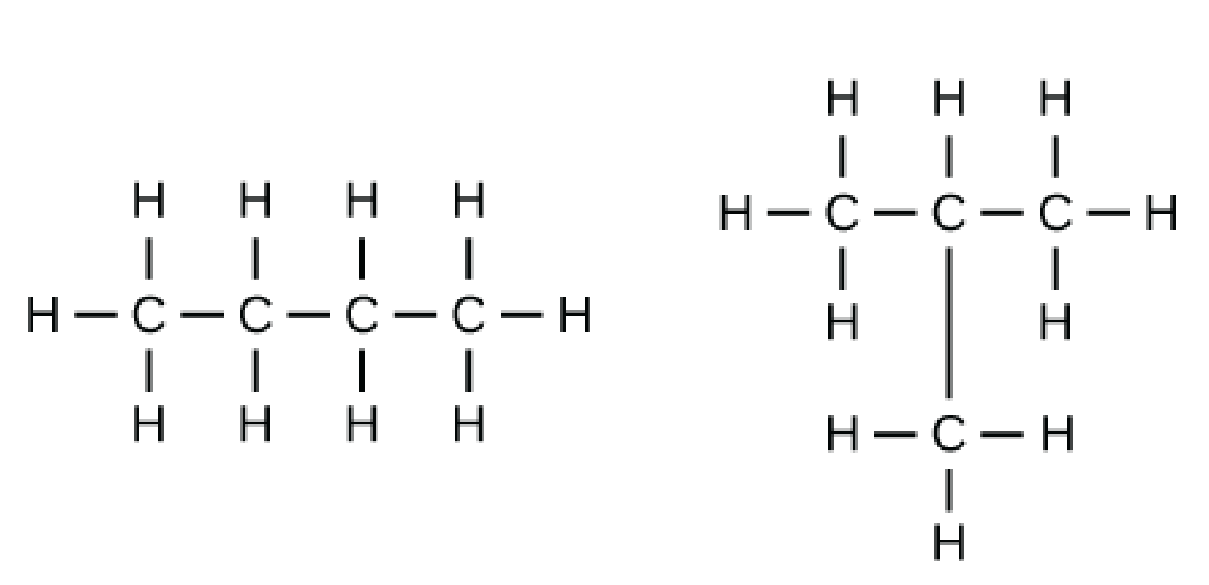
\includegraphics[scale = 0.105]{imagenes/hidrocarburo.png}
		\end{center}
		\pause
		
		\textbf{Soluci\'on}: La cantidad de v\'ertices es $p+q$. Por ser una mol\'ecula el grafo es conexo (si no es conexo ser\'ian 2 o m\'as mol\'eculas). Como no se forman ciclos, entonces el grafo con el que se modela la mol\'ecula es un \'arbol y por lo tanto tiene $p+q-1$ aristas.
		\pause
		
		Usando la f\'ormula de la suma de los grados, concluimos que: $$ 4p + q = 2(p+q-1) \iff q = 2p + 2$$
	\end{minipage}
\end{frame}

\begin{frame}{Árbol generador}
    \begin{itemize}
        \item Repaso: sea $\mathcal{G}=(V_G,E_G)$, $\mathcal{H}=(V_H, E_H)$ es un subgrafo de $\mathcal{G}$ si $V_H\subseteq V_G$ y $E_H \subseteq E_G$.
        \item Repaso: $\mathcal{H}$ es subgrafo generador de $\mathcal{G}$ si $V_H=V_G$.
        \item Un árbol generador de $\mathcal{G}$ es un subgrafo generador de $\mathcal{G}$ que es un árbol.
    \end{itemize}
    
    \begin{figure}
        \centering
        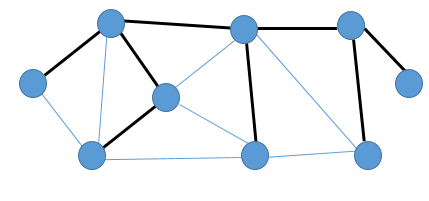
\includegraphics[width=\textwidth]{imagenes/edges_spinning_tree.jpg}
    \end{figure}
\end{frame}

\begin{frame}{Ejercicio 4}
	\begin{minipage}{\anchoPagina \textwidth}
	    \footnotesize
		Se tienen $N$ ciudades y $M$ rutas que las conectan. En el plano original es posible llegar de cualquier ciudad a otra mediante combinaciones de rutas.
		
		Las ciudades se dividen en dos grupos. Hay $A$ del grupo 1 y $B$ del grupo 2 (o sea que $A + B = N$). Se quiere renovar el pavimento de algunas rutas de forma tal que de todas las ciudades de grupo 1 se llegue a alguna ciudad de grupo 2 usando solamente rutas con pavimento renovado. ¿Cu\'al es la menor cantidad de rutas que hacen falta pavimentar?
		\begin{center}
			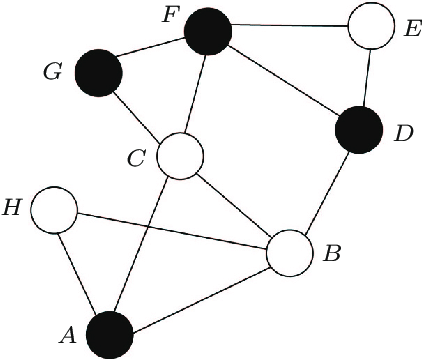
\includegraphics[scale = 0.36]{imagenes/blanco-negro.png}
		\end{center}
	\end{minipage}
\end{frame}

\begin{frame}{Ejercicio 4}
	\begin{minipage}{\anchoPagina \textwidth}
		\begin{center}
			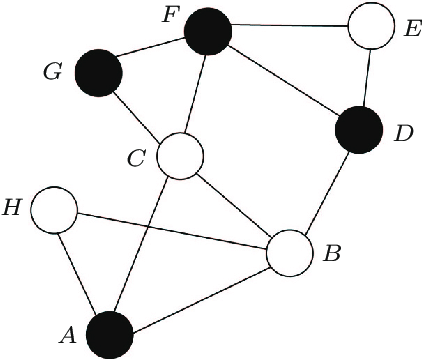
\includegraphics[scale = 0.36]{imagenes/blanco-negro.png}
		\end{center}
		
		\pause
		
		\textbf{Soluci\'on}: De cada ciudad del grupo 1, necesariamente vamos a tener que pavimentar alguna ruta que se conecte con ella (en caso contrario, esa ciudad jam\'as podr\'a llegar a una del grupo 2). Por lo tanto, debemos pavimentar al menos $A$ rutas. ¿Podemos lograr nuestro objetivo utilizando solo $A$ rutas? 
		\pause 
		
		¿Hace falta que el grafo original sea conexo? ¿C\'omo podemos verlo usando lo que vimos hasta ahora?
	\end{minipage}
\end{frame}

\begin{frame}{Repaso de definiciones}
	\begin{minipage}{\anchoPagina \textwidth}
		\begin{itemize}
			\item Un grafo $\mathcal{G} = (\mathbb{V},\mathbb{E},w)$ se dice \textit{pesado} si sus aristas tienen asociadas un cierto n\'umero, dado por $w : \mathbb{E} \to \mathbb{R}$
			\pause
			\item $\mathcal{T}$ es un \'arbol \textit{generador m\'inimo}  de $\mathcal{G}$, si es un subgrafo de $\mathcal{G}$ que es \'arbol (conexo y ac\'iclico), generador ($\mathbb{V}_{\mathcal{T}} = \mathbb{V}$) y minimiza $\sum\limits_{e \in \mathbb{E}_{\mathcal{T}}} w(e)$
			\pause
			\item El \textit{cuello de botella} de un \'arbol se define como $\underset{e \in \mathbb{E}_{\mathcal{T}}}{\max} w(e)$
		\end{itemize}
		\pause
		\begin{center}
			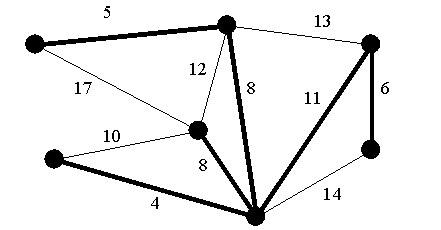
\includegraphics[scale = 0.55]{imagenes/mst.png}
		\end{center}
	\end{minipage}	
\end{frame}

\begin{frame}{Ejercicio 5}
	\begin{minipage}{\anchoPagina \textwidth}
		Se tienen $N$ ciudades y $M$ rutas que conectan un par de ciudades. Las ciudades se dividen en dos grupos. Hay $A$ del grupo 1 y $B$ del grupo 2 (o sea que $A + B = N$). Se quiere renovar el pavimento de algunas rutas de forma tal que de todas las ciudades de grupo 1 se llegue a alguna ciudad de grupo 2 usando solamente rutas con pavimento renovado. Cada ruta $e$ tiene un costo $w_e$ ¿Cu\'al es el menor costo con el que se puede lograr el objetivo?
		
		\begin{center}
			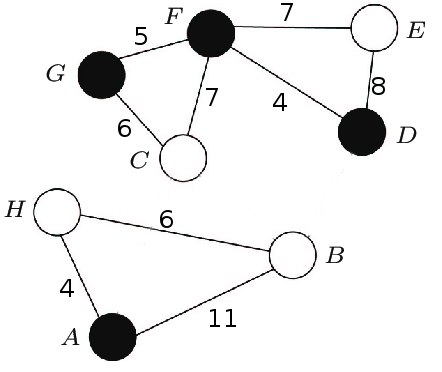
\includegraphics[scale = 0.29]{imagenes/blanco-negro-2.png}
		\end{center}
% 		\pause
% 		¿Se modifica la soluci\'on en caso de haber aristas negativas?	
	\end{minipage}
\end{frame}

% \begin{frame}{Ejercicio 2 - Problema del viajante de comercio}
% 	\begin{minipage}{\anchoPagina \textwidth}
% 		Sea $\mathcal{G}$ el grafo dado por $n$ ciudades entre las que podemos viajar entre cualquier par de ciudades. La distancia entre un par de ciudades $i,j$ est\'a dada por $d_{ij} \geq 0$. Dado un subgrafo $\mathcal{H}$, llamamos $w(\mathcal{H})$ a la suma de las distancias/pesos en las aristas de $\mathcal{H}$. Se busca encontrar un ciclo simple que minimice $w$.
		
% 		\medskip
% 		\pause
% 		\textbf{Problema 1}: Sea $\mathcal{C}$ la soluci\'on al problema del viajante de comercio y $\mathcal{T}$ el \'arbol generador m\'inimo del grafo. Probar que $w(\mathcal{T}) \leq w(\mathcal{C})$
		
% 		\medskip
% 		\pause
% 		\textbf{Problema 2}: Si las distancias cumplen con la desigualdad triangular, probar ahora que: $w(\mathcal{C}) \leq 2 w(\mathcal{T})$
% 		\pause
% 		\begin{center}
% 			
\includegraphics[scale = 0.19]{TSP-MST.png}
% 		\end{center}
% 	\end{minipage}
% \end{frame}

\begin{frame}{\'Arbol enraizado}
	\begin{minipage}{\anchoPagina \textwidth}
		\begin{itemize}
			\item $\mathcal{T}$ es un \'arbol \textit{enraizado} si distinguimos a un nodo de $\mathcal{T}$ al cual llamamos la \textit{ra\'iz}.
			\pause
			\item Puede ser dirigido o no. En caso de ser dirigido, hay dos formas naturales en las que se dirigen las aristas que son acerc\'andose a la ra\'iz o alej\'andose de la ra\'iz.
			\pause
			\item Definimos la \textit{profundidad} de un nodo como la distancia a la ra\'iz.
			\pause
			\item La \textit{altura} de un \'arbol enraizado est\'a dada por la m\'axima profundidad en el \'arbol.
			\pause
			\item Si un v\'ertice $v$ es un predecesor en un camino desde la ra\'iz a otro v\'ertice $w$, decimos que $v$ es el \textit{padre} de $w$ (y que $w$ es un hijo de $v$). A dos v\'ertices que tienen un mismo padre se los llaman \textit{hermanos}.
			\pause
			\item Un v\'ertice $v$ es un \textit{ancestro} de $w$ si $v$ se encuentra en el camino que une a la ra\'iz con $w$. Adem\'as en este caso, se dice que $w$ es un descendiente de $v$.
			
		\end{itemize}
	\end{minipage}
	
\end{frame}

\begin{frame}{\'Arbol enraizado}
	\begin{minipage}{\anchoPagina \textwidth}
	    \footnotesize
		\begin{itemize}
			\item Un v\'ertice que no tiene hijos se lo llama una \textit{hoja}. Todo v\'ertice que tenga al menos un hijo se lo llama \textit{interno}.
			\pause
			
			\item Un \'arbol enraizado se dice $\textit{k-ario}$, si todo v\'ertice tiene a lo sumo $k$ hijos. Si todas las hojas tienen la misma altura, y todo v\'ertice que no es hoja tiene exactamente $k$ hijos, se dice que es un \textit{\'arbol k-ario completo}
			
		\end{itemize}
		\begin{center}
			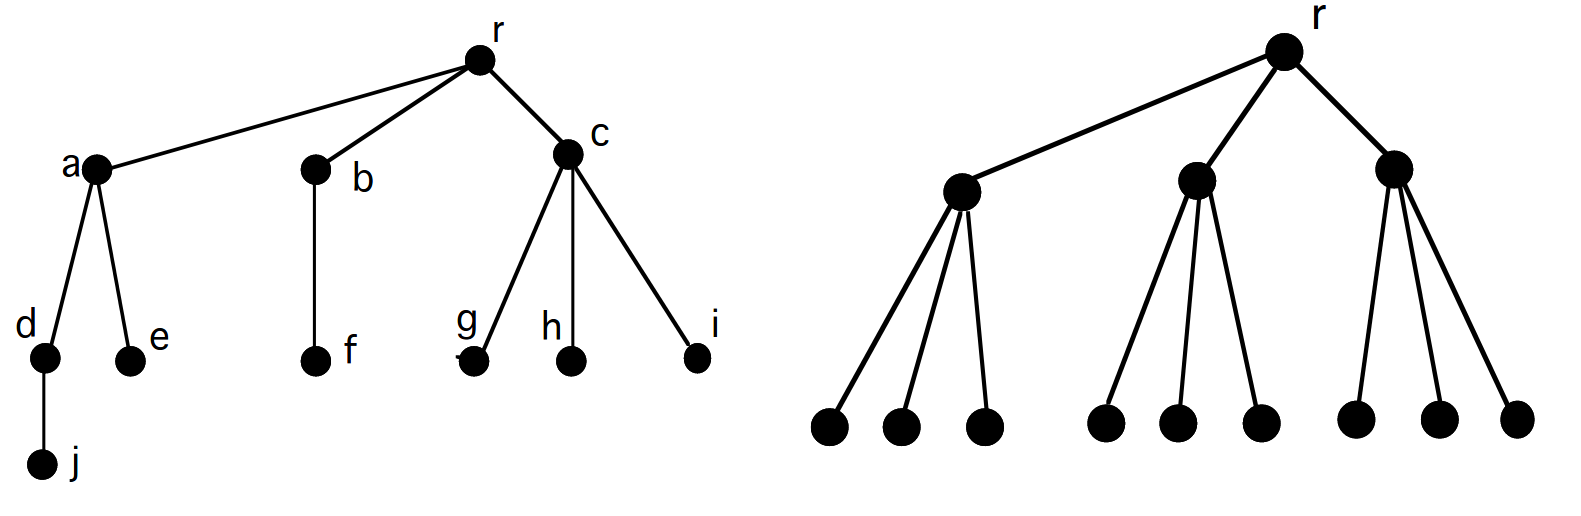
\includegraphics[scale = 0.16]{imagenes/root-tree-both.png}
		\end{center}
		\pause
		\textbf{Recordar}: la altura de un árbol $k$-ario completo con $n$ vértices es $O(log_k((k-1)m))$
		
		\vspace{2em}
		
		\textbf{Ejercicio}: Si $H$ e $I$ denotan la cantidad de hojas y de nodos internos respectivamente, probar que en un \'arbol $k$-ario completo, vale que $$H = (k-1)I + 1$$
	\end{minipage}
	
\end{frame}

\begin{frame}{\'Arbol binario de b\'usqueda}
	\begin{minipage}{\anchoPagina \textwidth}
	    \small
		Un \textit{\'arbol binario de b\'usqueda} guarda en cada nodo un valor. Es un \'arbol 2-ario que cumple que el sub\'arbol izquierdo de cualquier nodo (de existir) contiene valores menores que el del nodo en cuesti\'on, y el sub\'arbol derecho (de existir) valores mayores. 
		\pause
		\begin{center}
			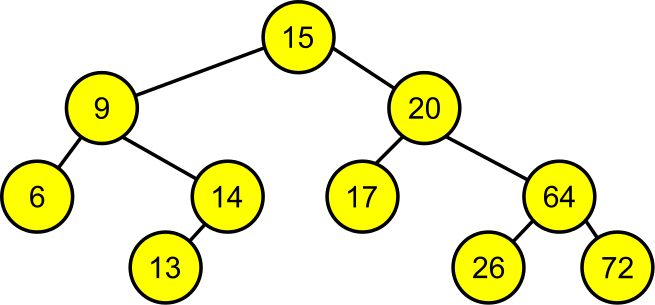
\includegraphics[scale = 0.3]{imagenes/ABB.png}
		\end{center}
		\pause
		\begin{itemize}
			 \item \textit{pre-order} (raíz, izq, der): \pause 15, 9, 6, 14, 13, 20, 17, 64, 26, 72
			 \pause
			 \item \textit{in-order} (izq, raíz, der): \pause 6, 9, 13, 14, 15, 17, 20, 26, 64, 72
			 \pause
			 \item \textit{post-order} (izq, der, raíz): \pause 6, 13, 14, 9, 17, 26, 72, 64, 20, 15
		\end{itemize}
		%\pause
		
% 		¿Cu\'antos \'arboles binarios de $n$ v\'ertices hay? \pause $\frac{1}{n+1} \binom{2n}{n}$, ¿por qu\'e?
	\end{minipage}

\end{frame}



\begin{frame}{Heap}
	\begin{minipage}{\anchoPagina \textwidth}
			
		Al igual que el \'arbol binario de b\'usqueda, un \textit{heap} es un \'arbol binario donde vamos a guardar valores en los nodos, pero el \'arbol binario en cuesti\'on es \textit{casi} completo (con excepci\'on del \'ultimo nivel, que se llena de izquierda a derecha). 
		
		En un \textit{max-heap} el valor de cada nodo es mayor al valor de cada uno de sus hijos. Dado un heap, podemos \textit{insertar} un nuevo valor, \textit{borrar} el mayor elemento (la ra\'iz), y \textit{consultar} el valor en la ra\'iz.
		\pause
		\begin{center}
			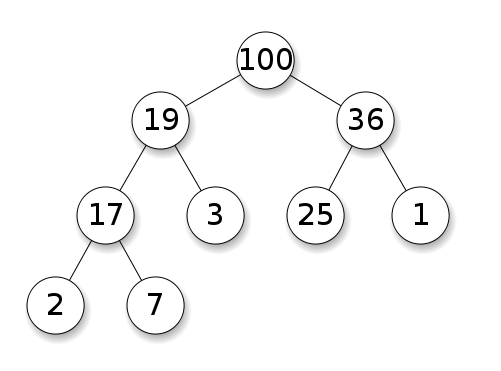
\includegraphics[scale = 0.23]{imagenes/max-heap.png}
		\end{center}
		
		\pause
		
		¿C\'omo implementar\'iamos cada una de ellas? ¿Qu\'e complejidades temporales tienen?
		
% 		\pause
		
% 		¿En qu\'e parte del algoritmo de Prim puede interesarnos un \textit{heap}?
	
	\end{minipage}	
	
\end{frame}

%\begin{frame}{Ejercicio}
%	
%	\pause
%	{\small 
%	El proceso de manufactura de una joya comienza con un pedazo de plata en bruto. La plata se tiene que \textit{tallar}, \textit{pulir}, \textit{agujerear} y \textit{marcar} de manera conveniente:
%	\begin{itemize}
%		\item Hay que tallarla antes que agujerearla.
%		\item Hay que pulirla antes que marcarla.
%	\end{itemize}
%	Adem\'as, cada proceso demora una cierta cantidad de tiempo.
%	\begin{itemize}
%		\item El proceso de tallado demora 1 unidad de tiempo.
%		\item El proceso de pulido demora 1 unidad de tiempo.
%		\item El proceso de marcado requiere de 2 unidades de tiempo si la pieza no est\'a tallada y 4 unidades de tiempo si la pieza est\'a tallada.
%		\item Agujerearla requiere de 3 unidades de tiempo si la pieza no est\'a pulida. Si la pieza est\'a pulida, pero no marcada, entonces agujerearla requiere de 5 unidades de tiempo. Por otro lado, si la pieza est\'a pulida y tambi\'en marcada, se requieren 7 unidades de tiempo para agujerearla.
%	\end{itemize}
	
%	Modelar el proceso mediante un grafo adecuado con el objetivo de realizar todos los procesos necesarios a la joya en cuesti\'on en el menor tiempo posible.
%	}
	
	
%\end{frame}




\end{document}

